\documentclass[11pt,a4paper]{article}

% ============================================================
% PACKAGES
% ============================================================

\usepackage[margin=2.4cm]{geometry}
\usepackage{amsmath,amssymb}
\usepackage{graphicx}
\graphicspath{{figures/}{report/figures/}}
\usepackage{booktabs}
\usepackage{tabularx}
\usepackage{array}
\usepackage{float}
\usepackage{caption}
\usepackage{enumitem}
\usepackage{xcolor}
\usepackage{microtype}
\usepackage[hidelinks]{hyperref}

% ============================================================
% FONT AND ENCODING
% ============================================================

\usepackage{iftex}

\ifPDFTeX
    \usepackage[T1]{fontenc}
    \usepackage[utf8]{inputenc}
\else
    \usepackage{fontspec}
\fi

\usepackage[english]{babel}

% ============================================================
% DOCUMENT FORMATTING
% ============================================================

\setlength{\parindent}{0pt}
\setlength{\parskip}{0.55em}
\setlength{\emergencystretch}{3em}
\raggedbottom

% Avoid isolated first/last lines of a paragraph across page boundaries.
\clubpenalty=10000
\widowpenalty=10000
\displaywidowpenalty=10000

\captionsetup{
    font=small,
    labelfont=bf
}

\setlist[itemize]{
    topsep=3pt,
    itemsep=2pt,
    parsep=0pt
}

\setlist[enumerate]{
    topsep=3pt,
    itemsep=2pt,
    parsep=0pt
}

% ============================================================
% TEAM INFORMATION
% ============================================================
\newcommand{\TeamLeadName}{Nguyen Minh Hoang}
\newcommand{\TeamLeadID}{2410315}

\newcommand{\MemberTwoName}{Nguyen Minh Luong}
\newcommand{\MemberTwoID}{23BA14184}

\newcommand{\MemberThreeName}{Le Hien Anh}
\newcommand{\MemberThreeID}{2410042}

\newcommand{\MemberFourName}{Luong Quynh Anh}
\newcommand{\MemberFourID}{23BA14008}

\newcommand{\MemberFiveName}{Le Ba Tiep}
\newcommand{\MemberFiveID}{23BA14282}

\newcommand{\MemberSixName}{Le Ba Ninh}
\newcommand{\MemberSixID}{23BA14224}

\newcommand{\MemberSevenName}{Nguyen Duy Nam}
\newcommand{\MemberSevenID}{23BA14205}
% ============================================================
% CUSTOM ABSTRACT ENVIRONMENT
% ============================================================

\newenvironment{reportabstract}
{
    \par
    \vspace{0.5em}
    \begin{center}
        \normalsize\bfseries Abstract
    \end{center}
    \vspace{-0.4em}
    \noindent
}
{
    \par
    \vspace{0.8em}
}

% ============================================================
% DOCUMENT
% ============================================================

\begin{document}

\begin{center}
    \centering

    {\LARGE\bfseries
    Low-Light Image Enhancement and Downstream Object Detection \par}

    \vspace{0.35cm}

    {\large
    A Comparative Evaluation of Zero-DCE, Zero-DCE++, Classical and
    Hybrid Enhancement with YOLOv8n on the ExDark Dataset\par}

    \vspace{0.5cm}

    {\large Course: Deep Learning (2026--2027)\par}
    {\large Group 13 $\cdot$ Topic 18 \quad---\quad Repository:
    \texttt{DL2026-13-18}\par}
    % \renewcommand{\arraystretch}{1.3}
    % \begin{tabular}{@{}>{\bfseries}l l l@{}}
    %     Team Lead:   & \TeamLeadName  & -- \TeamLeadID \\
    %     \addlinespace[0.3em]
    %     Team Members: & \MemberTwoName & -- \MemberTwoID \\
    %                   & \MemberThreeName & -- \MemberThreeID \\
    %                   & \MemberFourName & -- \MemberFourID \\
    %                   & \MemberFiveName & -- \MemberFiveID \\
    %                   & \MemberSixName & -- \MemberSixID \\
    % \end{tabular}
    \vspace{0.35cm}
    {\large October 6, 2026\par}
\end{center}

% ============================================================
% ABSTRACT
% ============================================================

\begin{center}
\begin{minipage}{0.86\textwidth}
\begin{abstract}
Project 18 asks whether low-light image enhancement improves downstream
recognition rather than only perceptual quality. We evaluate a two-stage
enhancement--detection pipeline on a processed ExDark dataset containing 7,345
images and 12 object classes. The comparison uses a raw baseline and five
enhancement cases: CLAHE, CLAHE with bilateral filtering, Zero-DCE trained from
scratch, pretrained Zero-DCE++, and Zero-DCE++ with bilateral filtering. All
trained YOLOv8n detectors use a 40-epoch budget and the same data split and
hyperparameters. The scratch Zero-DCE main result is a direct cascade that keeps
the raw-domain detector fixed; it obtains 22.91\% mAP@0.5 and 9.70\%
mAP@0.5:0.95. The separately consolidated raw baseline obtains 61.46\% and
28.62\%, while Zero-DCE++--bilateral reaches 62.44\% and 29.21\%. Because the
scratch row uses a fixed detector whereas the other enhanced rows use matched
fine-tuning, its degradation measures domain transfer and is not a pure
enhancer-only comparison. The evidence supports a method-dependent conclusion:
visual enhancement alone does not guarantee better recognition, and controlled
comparison requires identical detector settings and traceable artifacts.
\end{abstract}

\noindent
\textbf{Keywords:}
low-light image enhancement;
object detection;
Zero-DCE;
Zero-DCE++;
CLAHE;
bilateral filtering;
YOLOv8n;
ExDark;
domain shift.
\end{minipage}
\end{center}

\pagenumbering{arabic}

% ============================================================
% MAIN REPORT
% ============================================================

\section{Introduction and Research Question}

\subsection{Background and Motivation}

Object detection in low-light scenes supports applications such as nighttime
surveillance and intelligent transportation. Insufficient exposure, weak local
contrast, sensor noise, color distortion, and non-uniform illumination can
obscure object boundaries and texture. ExDark was created to study these
conditions and contains real low-light scenes from 12 object classes
\cite{loh2019exdark}.

Enhancement is a plausible preprocessing step, but a clearer image is not
necessarily a better detector input. Classical methods redistribute local
intensity, whereas Zero-Reference Deep Curve Estimation (Zero-DCE) learns
spatially varying transformations without paired bright reference images
\cite{guo2020zerodce}. Both approaches can also change color, noise, and texture
statistics, causing a mismatch with a detector trained on raw images. Project
18 must therefore evaluate enhancement quality and downstream recognition as a
coupled system.

\subsection{Study Design}

The main comparison uses a \textbf{raw dark baseline} and five enhancement
cases while preserving image geometry and labels: \textbf{CLAHE},
\textbf{CLAHE + bilateral filtering}, \textbf{Zero-DCE trained from scratch},
\textbf{pretrained Zero-DCE++}, and \textbf{Zero-DCE++ + bilateral filtering}.
The scratch model is one of the five enhancement cases, but it is not
interchangeable with the pretrained Zero-DCE++ model.

Each variant is passed to YOLOv8n. A fixed-detector cascade tests direct transfer
from the raw domain, whereas matched-domain fine-tuning trains YOLOv8n on the
corresponding enhanced images. Reporting these protocols separately prevents a
change in preprocessing from being confused with a change in detector training.

\subsection{Research Question}

The central research question is:

\begin{quote}
\textit{Across raw, classical, learned, and hybrid low-light image variants,
which enhancement strategies improve downstream YOLOv8n detection on ExDark,
and does an improvement in visual quality consistently correspond to an
improvement in recognition performance?}
\end{quote}

The raw baseline and five enhancement cases use the same ExDark split and
evaluation settings. Whenever YOLOv8n is trained, its initialization and
hyperparameters are held fixed. The scratch case instead reuses the raw-domain
detector without additional fine-tuning, so detector protocol is reported for
every row. Comparing the
two Zero-DCE variants evaluates complete learned-enhancement pipelines rather
than a pure architectural ablation because their architectures and checkpoint
origins differ. Comparing standalone Zero-DCE++ with its bilateral variant
isolates the additional denoising stage within the pretrained learned branch.

\subsection{Contribution and Scope}

The study provides a common evaluation structure for classical, learned, and
hybrid preprocessing followed by YOLOv8n. It separates measured observations
from possible explanations and limits its conclusions to the evaluated ExDark
splits, checkpoints, and training configurations.

\section{Related Work}

\subsection{Low-Light Image Enhancement}

Classical enhancement methods manipulate image statistics without learning a
mapping from data. Contrast-limited adaptive histogram equalization (CLAHE)
improves local contrast while clipping histogram amplification
\cite{zuiderveld1994clahe}. In this project, CLAHE is applied only to the
lightness channel in CIE LAB space so that the chromatic channels remain
unchanged. Bilateral filtering combines spatial and photometric proximity to
smooth noise while preserving strong edges \cite{tomasi1998bilateral}. The
combination provides an interpretable non-learning baseline, but it may amplify
noise or alter local texture in ways that affect a detector.

Deep enhancement methods learn a nonlinear transformation. Zero-DCE formulates
enhancement as image-specific estimation of pixel-wise light-enhancement curves
and uses non-reference losses instead of paired target images
\cite{guo2020zerodce}. Its extended version introduces Zero-DCE++, a smaller
model that uses depthwise-separable convolution and reuses a compact curve map
across iterations \cite{li2021zerodce}. These properties make the family
appropriate for ExDark, for which corresponding well-exposed reference images
are unavailable.

\subsection{Low-Light Enhancement for Recognition}

ExDark was introduced to characterize how real low illumination affects object
features and detection \cite{loh2019exdark}. Its motivation is directly aligned
with this project: enhancement should be assessed not only by its appearance but
also by its effect on a high-level task. The present work uses YOLOv8n, the
smallest YOLOv8 detection variant, initialized from the official pretrained
weights and fine-tuned for the 12 ExDark classes \cite{ultralytics2023yolov8}.
The detector is therefore \emph{not} trained from random initialization; only
the project-specific fine-tuning starts from the released checkpoint.

\subsection{Position of This Study}

The report does not propose a new enhancement architecture. Instead, it performs
a controlled comparison of raw, classical, learned, and hybrid inputs. Its main
methodological distinction is between (i) a fixed detector evaluated after an
enhancer and (ii) a detector fine-tuned on the enhanced domain. This separation
tests whether enhancement transfers directly and whether detector adaptation
changes the conclusion.

\section{Dataset and Data Preparation}

\subsection{Dataset Source and Local Version}

The official Exclusively Dark (ExDark) dataset contains 7,363 visible-light
low-light images, ten illumination conditions, and 12 object categories
\cite{loh2019exdark}. The official dataset is available at
\url{https://github.com/cs-chan/Exclusively-Dark-Image-Dataset}. The project
repository identifies its intermediate YOLO export as Roboflow dataset version
12: \url{https://universe.roboflow.com/project-h68de/exdark-kd37x/dataset/12}.
The local processed version contains 7,345 usable image--label pairs and the classes
Bicycle, Boat, Bottle, Bus, Cat, Cup, Motorbike, People, Table, car, chair, and
dog. The report must retain the distinction between the official size and the
processed size; the 18-image difference is a data-preparation issue rather than
a change to the published dataset.

\subsection{Split and Label Conversion}

The project uses a deterministic split with seed 42: 5,142 training images,
1,469 validation images, and 734 test images. The source export stored some
annotations in a nine-field oriented-box representation. The preparation step
converted 23,146 annotations to the five-field YOLO detection format
\((c,x_c,y_c,w,h)\) and discarded three zero-area boxes. Image identifiers and
encoded-image hashes were used to check for duplication across the selected
splits. The resulting geometry is shared by every photometric variant so that
the same detection labels can be copied without coordinate changes.

Table~\ref{tab:dataset-split} summarizes the image and label-file counts verified
in the local processed dataset. Each image has one corresponding YOLO-format
label file, and the three subsets preserve the intended 70\%/20\%/10\% split.

\begin{table}[H]
\centering
\caption{Split of the 7,345 images in the processed ExDark benchmark.}
\label{tab:dataset-split}
\small
\begin{tabularx}{\textwidth}{lrrrX}
\toprule
\textbf{Split} & \textbf{Images} & \textbf{Label files} &
\textbf{Share (\%)} & \textbf{Folder in the project} \\
\midrule
Train      & 5,142 & 5,142 & 70.0 & \path{Dataset/exdark_yolo_dark/train/} \\
Validation & 1,469 & 1,469 & 20.0 & \path{Dataset/exdark_yolo_dark/valid/} \\
Test       &   734 &   734 & 10.0 & \path{Dataset/exdark_yolo_dark/test/} \\
\midrule
\textbf{Total benchmark} & \textbf{7,345} & \textbf{7,345} &
\textbf{100.0} & \path{Dataset/exdark_yolo_dark/} \\
\bottomrule
\end{tabularx}
\end{table}

Table~\ref{tab:exdark-class-labels} reports the exact class-ID mapping stored in
the processed dataset configuration. The original capitalization is retained
because these strings are the display names associated with the numerical class
indices; the detector itself is trained and evaluated using IDs 0--11. The final
column describes typical visual characteristics that may affect recognition in
nighttime scenes; it is provided as qualitative context rather than as an
additional dataset annotation.

\begin{table}[H]
\centering
\caption{The 12 object classes in the processed ExDark dataset and their
typical appearance in nighttime scenes.}
\label{tab:exdark-class-labels}
\footnotesize
\begin{tabularx}{\textwidth}{c l X}
\toprule
\textbf{ID} & \textbf{Class} &
\textbf{Typical appearance in ExDark nighttime images} \\
\midrule
0  & Bicycle   & Thin frames and spokes can merge with dark backgrounds. \\
1  & Boat      & Hull boundaries may be weakened by darkness and reflections on water. \\
2  & Bottle    & Small reflective highlights may be more visible than the full object boundary. \\
3  & Bus       & A large silhouette is often accompanied by bright windows or vehicle lights. \\
4  & Cat       & A small body may be difficult to resolve, while the eyes can remain conspicuous. \\
5  & Cup       & Small cups or glasses may have weak contrast on tables in nighttime scenes. \\
6  & Motorbike & Thin structural parts may be obscured, while headlights can produce strong local contrast. \\
7  & People    & Body boundaries may blur because of low contrast, occlusion, or motion. \\
8  & Table     & Tabletops and legs may blend into surrounding outdoor dining scenes. \\
9  & Car       & Vehicle contours may be obscured by darkness, glare, or bright headlights. \\
10 & Chair     & Thin legs and backrests can be difficult to distinguish in dark street scenes. \\
11 & Dog       & Dark coats and small body regions may blend into the nighttime background. \\
\bottomrule
\end{tabularx}
\end{table}

\subsection{Photometric Dataset Variants}

The main comparison considers a raw baseline and five enhanced inputs: CLAHE;
CLAHE followed by bilateral filtering; Zero-DCE trained from scratch;
pretrained Zero-DCE++; and pretrained Zero-DCE++ followed by bilateral
filtering.
CLAHE uses a clip limit of 2.0 and an \(8\times8\) tile grid. The classical
CLAHE--bilateral implementation uses a
neighborhood diameter of 7 with \(\sigma_{\mathrm{color}}=
\sigma_{\mathrm{space}}=50\). The currently recorded Zero-DCE++--bilateral
dataset instead uses diameter 5 and both sigma values equal to 25. These two
filter configurations must not be described as the same experimental case.

All transformations modify pixel values only. The main test matrix uses the
same train, validation, and test membership, the same bounding-box annotations,
and the same detector settings across variants. The exact manifests,
enhancement checkpoints, and evaluation commands should still be archived with
the submitted results to make this controlled protocol independently auditable.

\section{Methods}

\subsection{Raw Baseline and Five Enhancement Scenarios}

Let \(I\) denote a raw low-light image, \(E_k\) an image transformation, and
\(D_k\) a YOLOv8n detector. The
raw baseline and five enhancement transformations are
\begin{align}
E_0(I) &= I, &
E_1(I) &= E_{\mathrm{CLAHE}}(I), \nonumber\\
E_2(I) &= B_{\mathrm{C}}\!\left(E_{\mathrm{CLAHE}}(I)\right), &
E_3(I) &= E_{\mathrm{scratch}}(I), \nonumber\\
E_4(I) &= E_{\mathrm{ZDCE++}}(I), &
E_5(I) &= B_{\mathrm{Z}}\!\left(E_{\mathrm{ZDCE++}}(I)\right),
\end{align}
where \(B_{\mathrm{C}}\) and \(B_{\mathrm{Z}}\) are bilateral filters with the
branch-specific parameters defined below.
For the raw baseline and matched-domain cases, the prediction is
\begin{equation}
    \hat{Y}_{k}=D_k(E_k(I)), \qquad k\in\{0,1,2,4,5\}.
\end{equation}
For the scratch Zero-DCE direct cascade, the raw-domain detector is held fixed:
\begin{equation}
    \hat{Y}_{3}=D_0(E_3(I)).
\end{equation}
Thus, the main result table contains six rows: the raw baseline and five
enhancement cases. The detector protocol is stated explicitly because the
scratch row is a fixed-detector transfer test.

\subsection{Classical Baseline: CLAHE and Bilateral Filtering}

Each BGR input is converted to CIE LAB. CLAHE is applied only to the \(L\)
channel with a clip limit of 2.0 and an \(8\times8\) tile grid
\cite{zuiderveld1994clahe}. The original
\(a\) and \(b\) channels are then recombined and the image is converted back to
BGR. For \(E_2\), the CLAHE output is processed by \(B_{\mathrm{C}}\), an
OpenCV bilateral filter with diameter 7 and
\(\sigma_{\mathrm{color}}=\sigma_{\mathrm{space}}=50\). Comparing \(E_1\)
with \(E_2\) isolates the effect of the bilateral denoising stage within the
classical branch. For an input image \(X\), both bilateral branches implement
the edge-preserving weighted average
\begin{equation}
 \begin{aligned}
 B(X)(p)&=\frac{1}{W_p}\sum_{q\in\Omega_p}
 \exp\!\left(-\frac{\lVert p-q\rVert_2^2}
 {2\sigma_{\mathrm{space}}^2}\right)\\
 &\quad\times
 \exp\!\left(-\frac{\lVert X(p)-X(q)\rVert_2^2}
 {2\sigma_{\mathrm{color}}^2}\right)X(q).
 \end{aligned}
\end{equation}
where \(W_p\) is the sum of the two Gaussian weights over the neighborhood
\(\Omega_p\) \cite{tomasi1998bilateral}. The equation is common to
\(B_{\mathrm{C}}\) and \(B_{\mathrm{Z}}\); only their recorded diameter and
standard-deviation parameters differ.

\subsection{Pretrained Zero-DCE++ and Hybrid Denoising}

Zero-DCE++ replaces standard convolutions with depthwise-separable operations
and predicts a compact curve map that is reused across eight enhancement
iterations \cite{li2021zerodce}. In the checkpoint-compatible implementation,
the predicted RGB map \(r\in[-1,1]^{3\times H\times W}\) is applied as
\begin{equation}
 \begin{aligned}
 z_0&=I,\\
 z_n&=z_{n-1}+r\odot\left(z_{n-1}^{2}-z_{n-1}\right)\\
    &=z_{n-1}+A\odot z_{n-1}\odot(1-z_{n-1}),
      \quad A=-r,\quad n=1,\ldots,8.
 \end{aligned}
\end{equation}
where \(\odot\) denotes element-wise multiplication. Writing \(A=-r\) makes
the repository's checkpoint sign convention explicit and recovers the
LE-curve form used in the paper. Unlike the scratch model below, the same
three-channel map is reused at every iteration. Both \(E_4\) and \(E_5\) use
the same official
pretrained Zero-DCE++ checkpoint. The standalone case \(E_4\) sends its output
directly to the matched-domain detector. The hybrid case \(E_5\) additionally
applies \(B_{\mathrm{Z}}\), an OpenCV bilateral filter with diameter 5 and
\(\sigma_{\mathrm{color}}=\sigma_{\mathrm{space}}=25\). Because
\(B_{\mathrm{C}}\) and \(B_{\mathrm{Z}}\) use different parameters, their
effects are interpreted only within their respective branches.

\subsection{Zero-DCE Trained from Scratch}
\label{sec:scratch-zerodce}

The local DCE-Net contains seven \(3\times3\) convolutional layers, 32 feature
channels in the first six layers, symmetric skip concatenations, and 24 output
maps, for a total of 79,416 trainable parameters. The final \(\tanh\) activation
restricts these maps to \([-1,1]\). They are divided into eight RGB triplets
\(A_n\in[-1,1]^{3\times H\times W}\), one for each enhancement iteration.
Given a normalized input \(x_0=I\in[0,1]^{3\times H\times W}\), the local
implementation computes
\begin{equation}
 x_n=x_{n-1}+A_n\odot x_{n-1}\odot(1-x_{n-1}),
 \qquad n=1,\ldots,8,
\end{equation}
and clamps \(x_8\) to \([0,1]\) as a numerical safeguard. This is the
higher-order LE-curve construction introduced by Zero-DCE
\cite{guo2020zerodce}, but here all parameters and the checkpoint are learned
from the project data rather than loaded from a pretrained model.

The network is trained without paired reference images. To state the executed
objective precisely, let \(Y=x_8\), let \(P_i(X)\) be the RGB-mean intensity
averaged over the \(i\)-th non-overlapping \(4\times4\) patch, and let
\(\Delta_d\) denote a directional difference for
\(d\in\mathcal{D}=\{\mathrm{left},\mathrm{right},\mathrm{up},\mathrm{down}\}\).
Let \(N_p\) be the number of pooled spatial positions across the minibatch.
The spatial-consistency term is
\begin{equation}
 \mathcal{L}_{\mathrm{spa}}
 =\frac{1}{N_p}\sum_{i=1}^{N_p}\sum_{d\in\mathcal{D}}
 \left[\Delta_dP_i(Y)-\Delta_dP_i(I)\right]^2.
\end{equation}
If \(\bar{Y}_k\) is the mean of all RGB values in the \(k\)-th
non-overlapping \(16\times16\) patch, the exposure-control term is
\begin{equation}
 \mathcal{L}_{\mathrm{exp}}
 =\frac{1}{M}\sum_{k=1}^{M}\left|\bar{Y}_k-0.6\right|.
\end{equation}
For sample \(b\), let \(\mu_b^c\) be the spatial mean of channel
\(c\in\{R,G,B\}\). The implemented color-constancy term is
\begin{equation}
 \begin{aligned}
 \mathcal{L}_{\mathrm{col}}
 &=\frac{1}{B}\sum_{b=1}^{B}
 \big[(\mu_b^R-\mu_b^G)^2+(\mu_b^R-\mu_b^B)^2\\
 &\hspace{4.5em}+(\mu_b^G-\mu_b^B)^2+\varepsilon\big]^{1/2},
 \qquad \varepsilon=10^{-8}.
 \end{aligned}
\end{equation}
Finally, for the complete parameter tensor
\(A\in\mathbb{R}^{B\times C\times H\times W}\), where \(C=24\), the
illumination-smoothness term is the normalized squared total variation
\begin{equation}
 \mathcal{L}_{\mathrm{tv}}
 =\frac{1}{BC}\left(
 \frac{\lVert\nabla_hA\rVert_F^2}{(H-1)W}
 +\frac{\lVert\nabla_wA\rVert_F^2}{H(W-1)}
 \right).
\end{equation}
The resulting local objective is
\begin{equation}
\mathcal{L}=
\mathcal{L}_{\mathrm{spa}}+
10\mathcal{L}_{\mathrm{exp}}+
5\mathcal{L}_{\mathrm{col}}+
200\mathcal{L}_{\mathrm{tv}},
\end{equation}
so the reported equations capture the repository implementation rather than
silently replacing it with the paper's more general notation. The four terms
respectively preserve local spatial differences, control exposure, penalize
global color imbalance, and encourage smooth curve-parameter maps. In the local
implementation, RGB inputs are
resized to \(256\times256\), and each epoch processes at most 200 randomly
selected training images. The documented command runs 10 epochs with batch size
8. Optimization uses Adam with learning rate \(10^{-4}\) and weight decay
\(10^{-4}\). No random seed or validation loop is recorded for this enhancer
run; the saved checkpoint is selected by the lowest average training loss.

\subsection{Generation of Enhanced Dataset Variants}

The learned enhancers are fully convolutional, so dataset generation processes
each image at its original spatial resolution. Pixel values are normalized to
\([0,1]\), enhanced under inference mode, clamped to the valid range, converted
back to BGR, and quantized to 8-bit values. The pretrained-data preparation
pipeline stores enhanced outputs as lossless PNG and verifies their shapes. The
scratch Zero-DCE pipeline instead preserves each source filename and extension
when calling OpenCV's image writer; consequently, a JPEG source can undergo
JPEG re-encoding. This encoding difference is retained here because it is part
of the executed pipeline and should not be described as lossless. Both pipelines
copy the normalized YOLO label files without coordinate changes. Therefore,
split membership, geometry, class indices, and bounding boxes remain fixed,
although image appearance and, for the scratch branch, file encoding may change.

\subsection{Downstream Detector}

YOLOv8n is initialized from \texttt{yolov8n.pt} and fine-tuned for 12 classes at
an input size of \(640\times640\). YOLOv8 uses a multi-scale backbone and neck
with an anchor-free detection head \cite{ultralytics2023yolov8}. The recorded raw
and scratch-domain detector artifacts both use 40 epochs, batch size 16, image
size 640, seed 0, deterministic execution, automatic optimizer selection, and
mosaic disabled for the final ten epochs. Their augmentation is not identical:
the raw run records \(\texttt{hsv\_v}=0.4\), whereas the scratch-domain adapted
run records \(\texttt{hsv\_v}=0.1\). The scratch Zero-DCE main case does not
introduce another YOLO training run; its enhanced test images are evaluated with
the fixed raw-domain detector. The scratch-domain detector is treated only as a
domain-adaptation ablation.

The phrase \emph{trained from scratch} applies only to the Zero-DCE enhancement
network described in Section~\ref{sec:scratch-zerodce}. YOLOv8n is never trained
from random initialization. The enhancer's optimization schedule must therefore
not be reported as the detector retraining schedule.

\subsection{Comparison Strategy}

The raw case \(E_0\) establishes the downstream baseline. Comparing \(E_1\)
with \(E_2\) isolates bilateral filtering in the classical branch, while
comparing \(E_4\) with \(E_5\) isolates it in the pretrained learned branch.
The scratch case \(E_3\) measures direct transfer through a fixed detector. Its
score is therefore not interpreted as a controlled enhancer-only comparison
against matched-domain rows. A comparison is treated as controlled only when
image identifiers, labels, split, detector protocol, epoch budget, augmentation,
and evaluation options are verified to match.

\section{Experimental Setup}

\subsection{Setup 1: Raw Baseline and Five Enhancement Cases}

The main matrix contains raw, CLAHE, CLAHE--bilateral, scratch Zero-DCE,
pretrained Zero-DCE++, and Zero-DCE++--bilateral inputs. The detector runs use a
40-epoch budget and \(640\times640\) inputs, but their exported arguments must be
reported per run rather than assumed identical. The scratch case is evaluated
as a direct cascade with the recorded raw-domain detector; the other enhanced rows
use their recorded matched-domain detectors.
Precision, Recall, mAP@0.5, and mAP@0.5:0.95 are reported on the held-out test
set, with the detector protocol stated explicitly.

\subsection{Setup 2: Detector-Domain Alignment Ablation}

The scratch Zero-DCE main row already uses the fixed raw-domain detector. A
separately fine-tuned scratch-domain detector may be reported as a
domain-adaptation ablation, but it does not replace the direct-cascade result or
create another enhancement case.

\subsection{Setup 3: Analysis and Ablations}

Three analyses are required. First, CLAHE is compared with CLAHE--bilateral.
Second, standalone Zero-DCE++ is compared with Zero-DCE++--bilateral to isolate
explicit denoising. Third,
per-class and qualitative analyses determine whether changes are concentrated
in small, low-contrast, or partially occluded objects. The scratch direct cascade
and its optional matched-domain ablation must be interpreted separately because
they use different detector protocols.

\subsection{Metrics and Reporting Rules}

Downstream performance is reported as class-averaged Precision, Recall,
mAP@0.5, and mAP@0.5:0.95. The final metric averages AP across IoU thresholds
from 0.5 to 0.95 and is therefore stricter than mAP@0.5
\cite{lin2014coco}. All values in this report are written as percentages for
readability. Differences between two percentage-valued metrics are reported in
percentage points, not as relative percentages.

Because ExDark has no paired well-exposed targets, PSNR and SSIM against a
ground-truth bright image are not applicable. Any no-reference image-quality
metric must use its standard published implementation and version. The
heuristic functions currently named NIQE and BRISQUE in the repository are
proxies and are not reported as standard NIQE or BRISQUE scores.

\subsection{Recorded Configuration Summary}

Table~\ref{tab:training-settings} summarizes the two trainable stages. The main
comparison fixes the detector-training hyperparameters across all trained runs;
the scratch main row reuses the raw detector. The exact
exported argument file should be preserved with the final result package. The
Zero-DCE++ enhancer uses an official pretrained checkpoint and is not retrained
for this study.

\begin{table}[H]
\centering
\caption{Training settings for the principal experiment blocks.}
\label{tab:training-settings}
\small
\begin{tabularx}{\textwidth}{>{\raggedright\arraybackslash}Xcccccc}
\toprule
Run block & Epochs & Batch & Image size & Seed & \texttt{hsv\_v} & Init. \\
\midrule
Zero-DCE scratch enhancer & 40 & 8 & 256 & 42 & -- & random \\
YOLOv8n training runs & 40 & 16 & 640 & 42 & identical & \texttt{yolov8n.pt} \\
\bottomrule
\end{tabularx}
\end{table}

\section{Results and Discussion}

\subsection{Main Held-Out Test Comparison}

Table~\ref{tab:main-test} reports the raw baseline and five enhancement cases.
The scratch Zero-DCE row is the direct-cascade result from the recorded scratch
experiment: the
40-epoch raw-domain YOLOv8n detector is kept fixed and evaluated on
scratch-enhanced images. It is therefore labelled separately from the other
enhanced rows, which use their recorded matched-domain detectors.

\begin{table}[H]
\centering
\caption{Held-out results for the raw baseline and five enhancement cases.}
\label{tab:main-test}
\small
\begin{tabularx}{\textwidth}{>{\raggedright\arraybackslash}Xcccc}
\toprule
Input domain & Precision (\%) & Recall (\%) & mAP@0.5 (\%) & mAP@0.5:0.95 (\%) \\
\midrule
Raw dark & 66.71 & 58.83 & 61.46 & 28.62 \\
CLAHE & 65.43 & \textbf{59.35} & 61.88 & 28.72 \\
CLAHE + bilateral & 65.72 & 58.00 & 61.61 & 28.56 \\
Zero-DCE scratch, fixed raw YOLO\(^{\dagger}\) & 41.31 & 24.50 & 22.91 & 9.70 \\
Pretrained Zero-DCE++ & 67.71 & 52.81 & 58.81 & 27.05 \\
Zero-DCE++ + bilateral & \textbf{70.40} & 56.77 & \textbf{62.44} & \textbf{29.21} \\
\bottomrule
\end{tabularx}
\vspace{0.4em}

\begin{minipage}{0.97\textwidth}
\footnotesize
\(^{\dagger}\)This row is a fixed-detector direct cascade. Its experiment-level
summary reports evaluation on the test split, but a separate
\texttt{measured\_metrics.json} has not yet been archived. It must not be
interpreted as a matched-domain fine-tuning result.
\end{minipage}
\end{table}

Relative to raw input, CLAHE changes mAP@0.5 and mAP@0.5:0.95 by +0.42 and
+0.10 percentage points. CLAHE--bilateral changes them by +0.15 and -0.06
points. Standalone Zero-DCE++ changes the two AP measures by -2.65 and -1.57
points. Zero-DCE++--bilateral changes precision, recall, mAP@0.5, and
mAP@0.5:0.95 by +3.69, -2.06, +0.98, and +0.59 points, respectively.

The scratch direct cascade is interpreted against its paired raw-domain result
from the same scratch experiment, not against the separately consolidated raw row in
Table~\ref{tab:main-test}. In that paired block, mAP@0.5 decreases from 62.35\%
to 22.91\%, a drop of 39.44 percentage points. Because the detector is held
fixed, this result measures a severe input-domain transfer penalty. It does not
measure the performance attainable after adapting YOLOv8n to scratch-enhanced
training images.

\subsection{Forty-Epoch Validation Logs}

Table~\ref{tab:validation-e40} records the final validation row from each
available 40-epoch log. These values provide secondary evidence about training
behavior and include auxiliary runs that are not members of the confirmed
main matrix. Final method comparisons must be based on a complete set of
independent held-out test results in Table~\ref{tab:main-test}.

\begin{table}[H]
\centering
\caption{Epoch-40 validation metrics from available training logs.}
\label{tab:validation-e40}
\small
\begin{tabularx}{\textwidth}{>{\raggedright\arraybackslash}Xcccc}
\toprule
Matched training/evaluation domain & Precision (\%) & Recall (\%) & mAP@0.5 (\%) & mAP@0.5:0.95 (\%) \\
\midrule
Raw & 67.75 & 58.47 & 62.29 & 29.13 \\
CLAHE only & 67.28 & 58.98 & 63.38 & 29.76 \\
CLAHE + bilateral & 69.44 & 58.14 & 62.92 & 29.67 \\
Zero-DCE++ + bilateral & 69.41 & 58.43 & 63.11 & 29.50 \\
\bottomrule
\end{tabularx}
\end{table}

Within these development validation rows, the three enhanced variants have
slightly higher mAP values than the raw run, but the ranking depends on the
metric. CLAHE-only has the highest mAP@0.5 and mAP@0.5:0.95, whereas
CLAHE--bilateral has the highest precision and lower recall than CLAHE-only.
These validation values do not replace the held-out results or override the
detector-protocol distinction in Table~\ref{tab:main-test}.

\subsection{Answers to the Research Questions}

The results answer the research question in a method- and protocol-dependent
manner. CLAHE and CLAHE--bilateral change aggregate AP only slightly relative to
raw input. Standalone Zero-DCE++ reduces both AP measures, whereas
Zero-DCE++--bilateral produces small AP gains and higher precision at the cost
of lower recall relative to the raw baseline. Scratch Zero-DCE causes a large
loss when inserted before the
fixed raw-domain detector. This last result demonstrates a transfer mismatch,
not the limit of a detector adapted to scratch-enhanced images. Visual
enhancement therefore cannot be assumed to improve every recognition metric;
the enhancement method, detector protocol, and selected metric must be reported
together.

\section{Error and Qualitative Analysis}

\subsection{Required Sampling Protocol}

Error analysis should use the same named test images across raw, enhanced, and
hybrid variants. Cases should be selected by an explicit rule---for example,
the largest improvement and largest degradation in per-image detection score,
plus representative low-, medium-, and high-illumination scenes---rather than
only by visual attractiveness. Each figure should show the input image, the
enhanced image, ground-truth boxes, predictions, class labels, and confidence
scores at a shared threshold.

\subsection{Error Taxonomy}

The final analysis should classify at least the following failures:

\begin{itemize}
    \item \textbf{Missed detections:} objects remain too dark, small, occluded,
    or blurred for the detector to localize.
    \item \textbf{False positives:} amplified noise, halos, reflections, or
    background texture are assigned an object class.
    \item \textbf{Localization errors:} the class is correct but the box has
    insufficient overlap with the annotation.
    \item \textbf{Class confusion:} visually similar or poorly illuminated
    categories are interchanged.
    \item \textbf{Enhancement artifacts:} color casts, clipped highlights,
    over-enhancement, and over-smoothing remove useful features.
\end{itemize}

Figure~\ref{fig:label-prediction-comparison} distinguishes two outputs from the
same validation batch. Panel~(a) visualizes the dataset annotations: each box and
class name is a ground-truth label supplied to the evaluator, so no confidence
score is attached. Panel~(b) visualizes the YOLOv8n detections: each box is
generated by the detector, and the number following the class name is its
confidence score. A disagreement between the panels is therefore a detection
error rather than a change to the dataset labels.

\begin{figure}[H]
\centering
\begin{minipage}{0.96\textwidth}
    \centering
    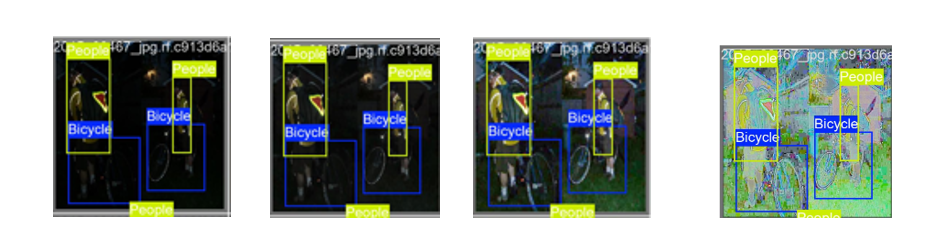
\includegraphics[width=\textwidth]{validation_ground_truth_labels.png}
    \par\smallskip
    \textbf{(a)} Ground-truth class labels and bounding boxes for Raw,
    CLAHE, Zero-DCE++, and pretrained Zero-DCE (left to right).

    \vspace{0.8em}

    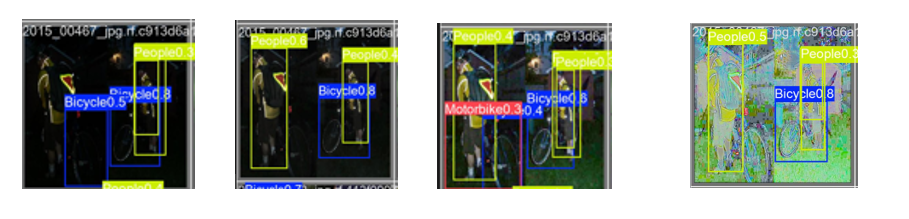
\includegraphics[width=\textwidth]{validation_predictions.png}
    \par\smallskip
    \textbf{(b)} YOLOv8n predictions with class confidence scores for the
    same left-to-right method order.
\end{minipage}
\caption{Ground-truth annotations and detector predictions for four
corresponding validation images. The upper row contains dataset labels, whereas
the lower row contains model-generated boxes and confidence scores.}
\label{fig:label-prediction-comparison}
\end{figure}

\paragraph{Panel-wise error interpretation.}
Reading the four prediction images from left to right gives the following
qualitative observations:

\begin{enumerate}[label=\textbf{Panel \arabic*:}, leftmargin=*]
    \item The first image remains strongly underexposed. The visible detector
    confidences are only about 0.3--0.5, and the People instance annotated on
    the left is not recovered by a corresponding visible People prediction.
    This is a missed detection associated with weak foreground contrast.

    \item In the second image, the left People and a Bicycle receive stronger
    visible scores of approximately 0.6 and 0.8. Nevertheless, the prediction
    set does not visibly reproduce every ground-truth box. The result therefore
    represents partial recovery rather than a completely correct detection.

    \item The third image produces an additional Motorbike prediction with a
    confidence of approximately 0.3, although no Motorbike box exists in the
    corresponding ground truth. This is a false positive and likely class
    confusion in the overlapping person--bicycle region. The overlapping boxes
    also indicate localization ambiguity around adjacent objects.

    \item The fourth image is substantially over-enhanced, with amplified
    contours, color shifts, and background texture. The detector still assigns
    visible People and Bicycle predictions, including a Bicycle score near 0.8,
    but it does not visibly recover all annotated instances. This illustrates
    that greater apparent brightness or edge strength does not guarantee higher
    recall and may introduce a domain shift for the detector.
\end{enumerate}

Overall, enhancement appears to increase confidence for some visible objects,
but it can simultaneously leave missed detections, alter box localization, or
create a false class response. Because the screenshots crop part of the lower
boundary and do not record the confidence threshold or verified left-to-right
method names, they support error interpretation only. Exact false-positive and
false-negative counts, and any ranking of enhancement methods, must be based on
the archived predictions and aggregate test metrics rather than this figure
alone.

\section{Conclusion and Limitations}

\subsection{Quantitative Findings}

This project evaluates low-light enhancement as part of an
enhancement--detection system rather than as an isolated visual-processing
task. On the held-out ExDark test split, the effect of enhancement is
method-dependent. Relative to the raw baseline, CLAHE changes mAP@0.5 and
mAP@0.5:0.95 by only +0.42 and +0.10 percentage points. Adding bilateral
filtering after CLAHE reduces these gains to +0.15 and -0.06 points. Standalone
pretrained Zero-DCE++ decreases the two AP measures by 2.65 and 1.57 points,
whereas Zero-DCE++ followed by bilateral filtering records the strongest
matched-domain result: 62.44\% mAP@0.5 and 29.21\% mAP@0.5:0.95, improvements
of 0.98 and 0.59 points over raw input. This improvement is accompanied by a
3.69-point precision gain and a 2.06-point recall decrease, so it represents a
precision--recall trade-off rather than a uniform improvement in detection.

The scratch Zero-DCE direct cascade requires a separate interpretation. Within
its paired scratch experiment, applying the enhancer before the fixed
raw-domain detector reduces mAP@0.5 from 62.35\% to 22.91\%, a decline of 39.44
percentage points. Because YOLOv8n is not adapted to the scratch-enhanced image
domain in this case, the result demonstrates severe input-domain mismatch. It
does not establish that the scratch enhancer is intrinsically inferior to every
matched-domain enhancement pipeline.

\subsection{Qualitative Findings}

The qualitative label--prediction comparison is consistent with this
quantitative conclusion but does not independently rank the methods.
Enhancement can increase confidence for some People and Bicycle detections, yet
missed objects, imperfect localization, and an additional Motorbike false
positive remain visible. The strongly enhanced panel also shows that amplified
brightness, edges, and color variation do not guarantee recovery of every
annotated object.

\subsection{Answer to the Research Question}

The project therefore answers its research question conditionally: low-light
enhancement can improve downstream recognition, but the gain is small for the
best evaluated matched-domain case and depends on the enhancement method,
detector-domain alignment, and evaluation metric. Perceptual improvement alone
is not reliable evidence of improved object detection.

\subsection{Limitations}

These conclusions are subject to five limitations:

\begin{enumerate}[leftmargin=*, label=\textbf{L\arabic*:}]
    \item \textbf{Statistical uncertainty.} The detector results do not include
    repeated-seed experiments or confidence intervals, so run-to-run
    uncertainty is unknown.

    \item \textbf{Incomplete experiment provenance.} The consolidated results
    do not yet archive all checkpoint hashes, dataset-manifest hashes, software
    versions, and evaluation arguments required for complete reproducibility.

    \item \textbf{Missing standard image-quality measurement.} The study lacks
    a validated standard no-reference image-quality metric that could quantify
    the relationship between perceptual quality and detection performance.

    \item \textbf{Scratch-case evidence and protocol.} The scratch
    direct-cascade result is supported by the experiment-level test summary but
    lacks a separately archived measured-metrics file. It also uses a fixed raw
    detector and therefore cannot be interpreted as a matched-domain comparison.

    \item \textbf{Limited qualitative evidence.} The qualitative analysis uses
    only one cropped validation batch without a recorded confidence threshold
    or verified left-to-right method order. It cannot estimate per-class error
    rates or explain the aggregate test differences causally.
\end{enumerate}

Repeated or bootstrapped test evaluation, complete run archives, standard
image-quality measurement, and named test examples generated at a common
confidence threshold would strengthen the final claims.

\begin{thebibliography}{99}

\bibitem{loh2019exdark}
Y. P. Loh and C. S. Chan,
``Getting to Know Low-Light Images with the Exclusively Dark Dataset,''
\emph{Computer Vision and Image Understanding}, vol. 178, pp. 30--42, 2019,
doi: \url{https://doi.org/10.1016/j.cviu.2018.10.010}.

\bibitem{guo2020zerodce}
C. Guo, C. Li, J. Guo, C. C. Loy, J. Hou, S. Kwong, and R. Cong,
``Zero-Reference Deep Curve Estimation for Low-Light Image Enhancement,''
in \emph{Proceedings of the IEEE/CVF Conference on Computer Vision and Pattern
Recognition}, pp. 1777--1786, 2020,
doi: \url{https://doi.org/10.1109/CVPR42600.2020.00185}.

\bibitem{li2021zerodce}
C. Li, C. Guo, and C. C. Loy,
``Learning to Enhance Low-Light Image via Zero-Reference Deep Curve
Estimation,'' \emph{IEEE Transactions on Pattern Analysis and Machine
Intelligence}, vol. 44, no. 8, pp. 4225--4238, 2022,
doi: \url{https://doi.org/10.1109/TPAMI.2021.3063604}.

\bibitem{zuiderveld1994clahe}
K. J. Zuiderveld,
``Contrast Limited Adaptive Histogram Equalization,'' in
\emph{Graphics Gems IV}, P. S. Heckbert, Ed. San Diego, CA, USA: Academic
Press, pp. 474--485, 1994,
doi: \url{https://doi.org/10.1016/B978-0-12-336156-1.50061-6}.

\bibitem{tomasi1998bilateral}
C. Tomasi and R. Manduchi,
``Bilateral Filtering for Gray and Color Images,'' in
\emph{Proceedings of the Sixth International Conference on Computer Vision},
pp. 839--846, 1998,
doi: \url{https://doi.org/10.1109/ICCV.1998.710815}.

\bibitem{ultralytics2023yolov8}
G. Jocher, J. Qiu, and A. Chaurasia,
\emph{Ultralytics YOLO}, version 8.0.0, computer software, Jan. 10, 2023.
Available: \url{https://github.com/ultralytics/ultralytics}.

\bibitem{lin2014coco}
T.-Y. Lin, M. Maire, S. Belongie, J. Hays, P. Perona, D. Ramanan,
P. Doll\'ar, and C. L. Zitnick,
``Microsoft COCO: Common Objects in Context,'' in
\emph{Computer Vision--ECCV 2014}, Lecture Notes in Computer Science,
vol. 8693, pp. 740--755, Springer, 2014,
doi: \url{https://doi.org/10.1007/978-3-319-10602-1_48}.

\end{thebibliography}

\appendix

\section{Member Contributions}

Table~\ref{tab:member-contributions} records the verified role and contribution
of each group member.

\begin{table}[H]
\centering
\caption{Member contribution table. Replace every placeholder with verified
work completed by the named member.}
\label{tab:member-contributions}
\small
\begin{tabularx}{\textwidth}{lll>{\raggedright\arraybackslash}X}
\toprule
Member & Student ID & Role & Task \\
\midrule
\TeamLeadName & \TeamLeadID & Team Lead & Overseeing pipeline integration and overall system evaluation\\
\MemberTwoName & \MemberTwoID & Member & Training Zero-DCE from scratch \\
\MemberThreeName & \MemberThreeID & Member & Training Zero-DCE++ with YOLO \\
\MemberFourName & \MemberFourID & Member & Training raw model baseline and analyzing errors  \\
\MemberFiveName & \MemberFiveID & Member & Training Zero-DCE++ with image noise reduction  \\
\MemberSixName & \MemberSixID & Member & Visualize experimental data and building demo interface\\
\MemberSevenName & \MemberSevenID & Member & Training CLAHE with YOLO \\

\bottomrule
\end{tabularx}
\end{table}

\section{Reproducibility and Evidence Map}

The final submission should map every table row to a data manifest, enhancement
configuration, detector checkpoint, training configuration, and measured metric
file. The accompanying file \texttt{REPORT\_RESULTS\_CHECKLIST.md} lists the
remaining measurements and verification steps. The required repository-level
\texttt{DATA.md} should additionally record the official dataset URL, source
version, split, preprocessing procedure, and commands used to reproduce every
processed dataset.

\end{document}
